% Mathematical and graphical reference: ../1-practice_activities/G11_T2_L1_C3_practice.tex
% User scope: retain the existing three independent exercises; exactly two tasks per problem.
\makeatletter
\def\input@path{{../../../preamble/}}
\makeatother
\input{preamble.tex}
\geometry{letterpaper,margin=0.25in}
\pagestyle{empty}
\linespread{1.04}
\setlength{\parskip}{4pt}
\raggedbottom
\newcommand{\stageheading}[1]{\par{\centering\large\bfseries #1\par}}
\newcommand{\problemtitle}[2]{\par\textbf{#1. #2}\par}
\newcommand{\task}[2]{\par\textbf{#1} #2\par}
\newenvironment{datagrid}[1]{\par\begingroup\small\setlength{\tabcolsep}{4pt}\setlength{\parskip}{0pt}\renewcommand{\arraystretch}{1.16}\tabularx{\linewidth}{#1}\hline}{\endtabularx\par\endgroup}
\pgfplotsset{relation/.style={width=.94\linewidth,height=7.4cm,axis lines=left,
 grid=major,major grid style={black!15},tick label style={font=\small},
 label style={font=\small},scaled ticks=false,enlargelimits=false,clip=true,
 tick label style={/pgf/number format/1000 sep={}}}}
% Reference label format, ordinary grayscale typography, five IDs per graph.
\newcommand{\PointLabel}[7]{%
 \node[font=\small,inner sep=2pt,anchor=#7] (point#1)
 at (axis description cs:#5,#6) {#1: $(#3,\,#4)$};
 \draw[black!70,line width=.35pt,shorten <=2.5pt] (axis cs:#2)--(point#1);
}
\newcommand{\LabelTemplates}{%
 \node[anchor=east,font=\small] at (axis description cs:.97,.93) {A: $(\underline{\hspace{.65cm}},\,\underline{\hspace{.65cm}})$};
 \node[anchor=east,font=\small] at (axis description cs:.97,.83) {B: $(\underline{\hspace{.65cm}},\,\underline{\hspace{.65cm}})$};
 \node[anchor=east,font=\small] at (axis description cs:.97,.73) {C: $(\underline{\hspace{.65cm}},\,\underline{\hspace{.65cm}})$};
 \node[anchor=east,font=\small] at (axis description cs:.97,.63) {D: $(\underline{\hspace{.65cm}},\,\underline{\hspace{.65cm}})$};
 \node[anchor=east,font=\small] at (axis description cs:.97,.53) {E: $(\underline{\hspace{.65cm}},\,\underline{\hspace{.65cm}})$};}
\newcommand{\workarea}{\begin{minipage}[t]{.49\linewidth}\vspace{0pt}
 \textbf{Calculation workspace}\par\smallskip
 \begin{tikzpicture}\draw[black!40] (0,0) rectangle (9.65,6.5);\end{tikzpicture}
 \end{minipage}}
\newcommand{\normalpanel}[2]{\begin{minipage}[t]{.32\linewidth}\vspace{0pt}\centering
 \textbf{$C=#1\%$}\par\medskip
 \begin{tikzpicture}\begin{axis}[width=.95\linewidth,height=5.4cm,
 xmin=-4,xmax=4,ymin=0,ymax=.46,enlargelimits=false,axis lines=left,
 xlabel={$z$ (unitless)},ylabel={Density},xtick={-#2,#2},
 xticklabels={$-#2$,$+#2$},ytick={0,.2,.4},
 tick label style={font=\small},label style={font=\small}]
 \addplot[draw=none,fill=black!18,domain=-#2:#2,samples=161]
 {exp(-x*x/2)/sqrt(2*pi)}\closedcycle;
 \addplot[black,thick,domain=-4:4,samples=201] {exp(-x*x/2)/sqrt(2*pi)};
 \draw[dashed] (axis cs:-#2,0)--(axis cs:-#2,.33)
 (axis cs:#2,0)--(axis cs:#2,.33);
 \node at (axis cs:0,.17) {$#1\%$};
 \end{axis}\end{tikzpicture}\par
 $-z^*=-#2,\quad +z^*=+#2$
 \end{minipage}}
\begin{document}
{\centering{\Large\bfseries C3: Anatomy of a confidence interval\par}
Global Economics | Grade 11 | Term 2 | Lesson 1\par}
\textbf{C3} Identifies the components of a confidence interval, including point estimate, critical value, standard error, and margin of error, explaining how each component affects precision and reliability.

\stageheading{Worked example}\problemtitle{1}{Weekly household grocery spending}
An analyst estimates the district mean weekly household grocery bill. For the explanatory intervals, the common point estimate is $\bar{x}=84$ thousand COP.
\task{Task 1:}{Illustrate the relationships between standard error, margin of error, and sample size.}
Hold $\sigma=30$ thousand COP and $C=95\%$ ($z^*=1.960$) fixed. Assume a simple random sample of independent observations from a much larger population, known population SD, and a normal population or approximately normal sample mean.
Use $\mathrm{SE}=\sigma/\sqrt n$ and $\mathrm{MoE}=z^*\times\mathrm{SE}$. Cases A--E correspond, in order, to $n=25,100,400,900,1600$. Each of the three graphs uses these five cases and five coordinate labels. SE and MoE use thousand COP.
\textbf{Solution.} For A, $\mathrm{SE}=30/\sqrt{25}=6.000$ and $\mathrm{MoE}=1.960(6.000)=11.760$ thousand COP. The remaining substitutions supply the other plotted coordinates.
\begin{datagrid}{|l|r|X|X|}ID&$n$&SE (thousand COP)&MoE (thousand COP)\\\hline
A&25&$30/\sqrt{25}=6.000$&$1.960(6.000)=11.760$\\\hline
B&100&$30/\sqrt{100}=3.000$&$1.960(3.000)=5.880$\\\hline
C&400&$30/\sqrt{400}=1.500$&$1.960(1.500)=2.940$\\\hline
D&900&$30/\sqrt{900}=1.000$&$1.960(1.000)=1.960$\\\hline
E&1600&$30/\sqrt{1600}=0.750$&$1.960(0.750)=1.470$\\\hline
\end{datagrid}
\par\smallskip
\begin{minipage}[t]{.49\linewidth}\vspace{0pt}\centering\textbf{Standard error vs sample size}\par\smallskip
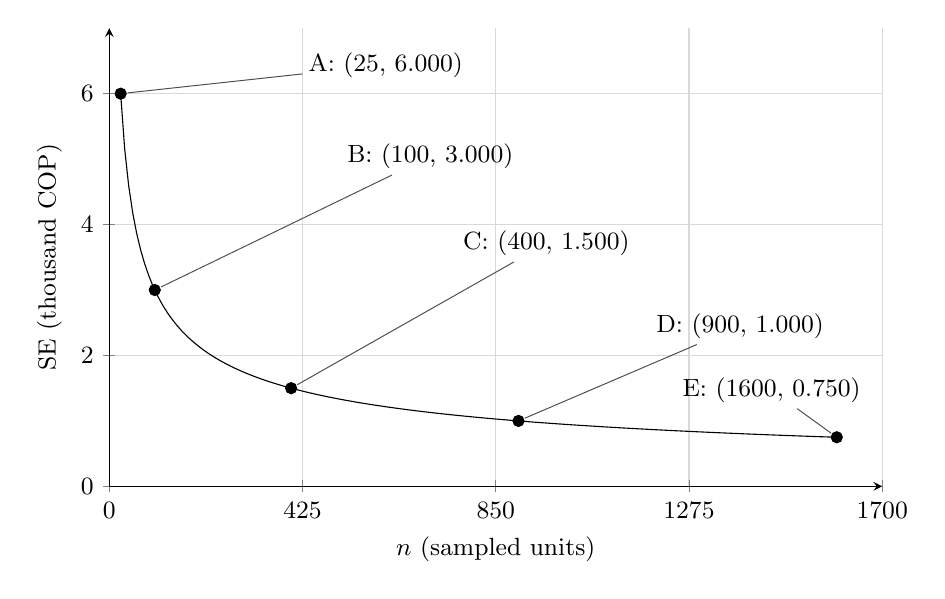
\begin{tikzpicture}\begin{axis}[relation,xlabel={$n$ (sampled units)},ylabel={SE (thousand COP)},xmin=0,xmax=1700,ymin=0,ymax=7,xtick={0,425,850,1275,1700}]
\addplot[black,domain=25:1600,samples=180] {30/sqrt(x)};
\addplot[only marks,mark=*,mark size=2pt] coordinates {(25.000000000,6.000000000) (100.000000000,3.000000000) (400.000000000,1.500000000) (900.000000000,1.000000000) (1600.000000000,0.750000000)};
\PointLabel{A}{25.000000000,6.000000000}{25}{6.000}{0.25}{0.92}{west}
\PointLabel{B}{100.000000000,3.000000000}{100}{3.000}{0.3}{0.72}{west}
\PointLabel{C}{400.000000000,1.500000000}{400}{1.500}{0.45}{0.53}{west}
\PointLabel{D}{900.000000000,1.000000000}{900}{1.000}{0.7}{0.35}{west}
\PointLabel{E}{1600.000000000,0.750000000}{1600}{0.750}{0.98}{0.21}{east}
\end{axis}\end{tikzpicture}\end{minipage}
\hfill
\begin{minipage}[t]{.49\linewidth}\vspace{0pt}\centering\textbf{Margin of error vs sample size}\par\smallskip
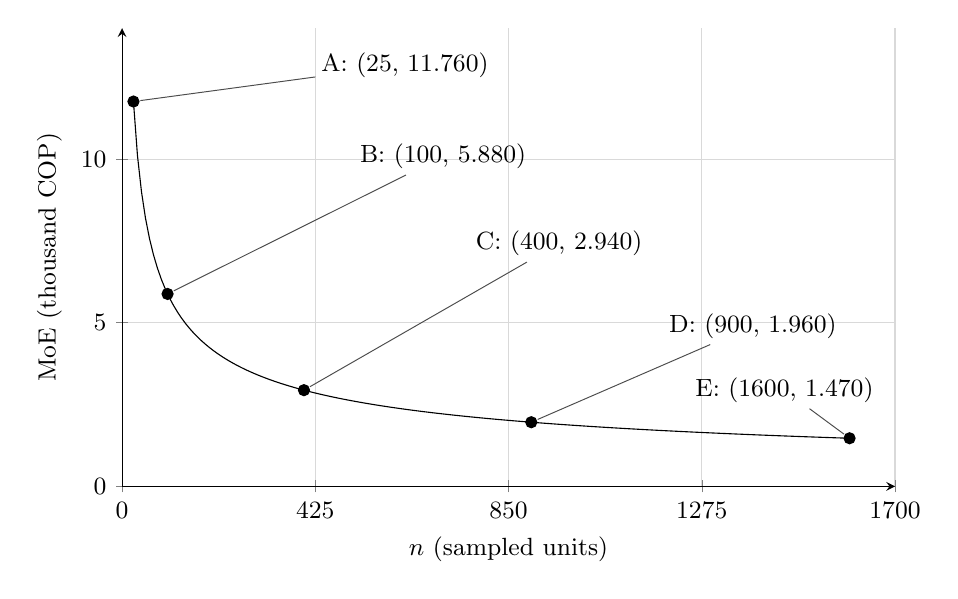
\begin{tikzpicture}\begin{axis}[relation,xlabel={$n$ (sampled units)},ylabel={MoE (thousand COP)},xmin=0,xmax=1700,ymin=0,ymax=14,xtick={0,425,850,1275,1700}]
\addplot[black,domain=25:1600,samples=180] {1.960*30/sqrt(x)};
\addplot[only marks,mark=*,mark size=2pt] coordinates {(25.000000000,11.760000000) (100.000000000,5.880000000) (400.000000000,2.940000000) (900.000000000,1.960000000) (1600.000000000,1.470000000)};
\PointLabel{A}{25.000000000,11.760000000}{25}{11.760}{0.25}{0.92}{west}
\PointLabel{B}{100.000000000,5.880000000}{100}{5.880}{0.3}{0.72}{west}
\PointLabel{C}{400.000000000,2.940000000}{400}{2.940}{0.45}{0.53}{west}
\PointLabel{D}{900.000000000,1.960000000}{900}{1.960}{0.7}{0.35}{west}
\PointLabel{E}{1600.000000000,1.470000000}{1600}{1.470}{0.98}{0.21}{east}
\end{axis}\end{tikzpicture}\end{minipage}
\par\medskip
\begin{minipage}[t]{.49\linewidth}\vspace{0pt}\centering\textbf{Margin of error vs standard error}\par\smallskip
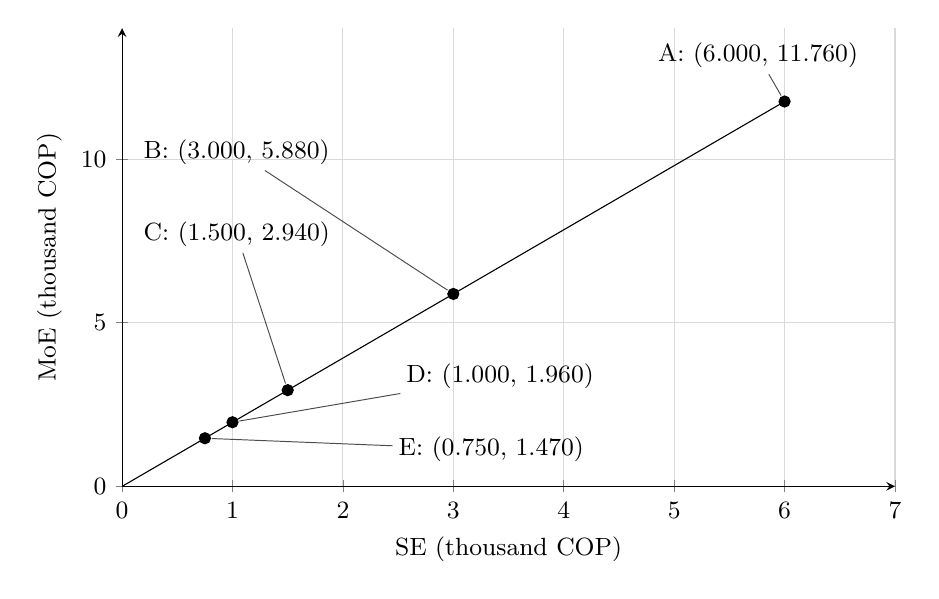
\begin{tikzpicture}\begin{axis}[relation,xlabel={SE (thousand COP)},ylabel={MoE (thousand COP)},xmin=0,xmax=7,ymin=0,ymax=14]
\addplot[black,domain=0:6.0] {1.960*x};
\addplot[only marks,mark=*,mark size=2pt] coordinates {(6.000000000,11.760000000) (3.000000000,5.880000000) (1.500000000,2.940000000) (1.000000000,1.960000000) (0.750000000,1.470000000)};
\PointLabel{A}{6.000000000,11.760000000}{6.000}{11.760}{0.96}{0.94}{east}
\PointLabel{B}{3.000000000,5.880000000}{3.000}{5.880}{0.02}{0.73}{west}
\PointLabel{C}{1.500000000,2.940000000}{1.500}{2.940}{0.02}{0.55}{west}
\PointLabel{D}{1.000000000,1.960000000}{1.000}{1.960}{0.36}{0.24}{west}
\PointLabel{E}{0.750000000,1.470000000}{0.750}{1.470}{0.35}{0.08}{west}
\end{axis}\end{tikzpicture}\end{minipage}
\par\clearpage
\textbf{Problem 1 --- Task 1 solution continued}\par
Both SE and MoE decrease as $n$ increases because they are proportional to $1/\sqrt n$. The continuous sample-size curves guide the eye between integer sizes. MoE vs SE is a line through the origin with slope $1.960$; confidence and population SD stay fixed.

\textbf{Explanatory confidence-interval comparison}\par
These three intervals use $\bar{x}\pm\mathrm{MoE}=84\pm1.960(30/\sqrt n)$, in thousand COP:
\[
\begin{aligned}
n=25:&\quad84\pm11.760=[72.240,95.760],\\
n=400:&\quad84\pm2.940=[81.060,86.940],\\
n=1600:&\quad84\pm1.470=[82.530,85.470].
\end{aligned}
\]
\begin{center}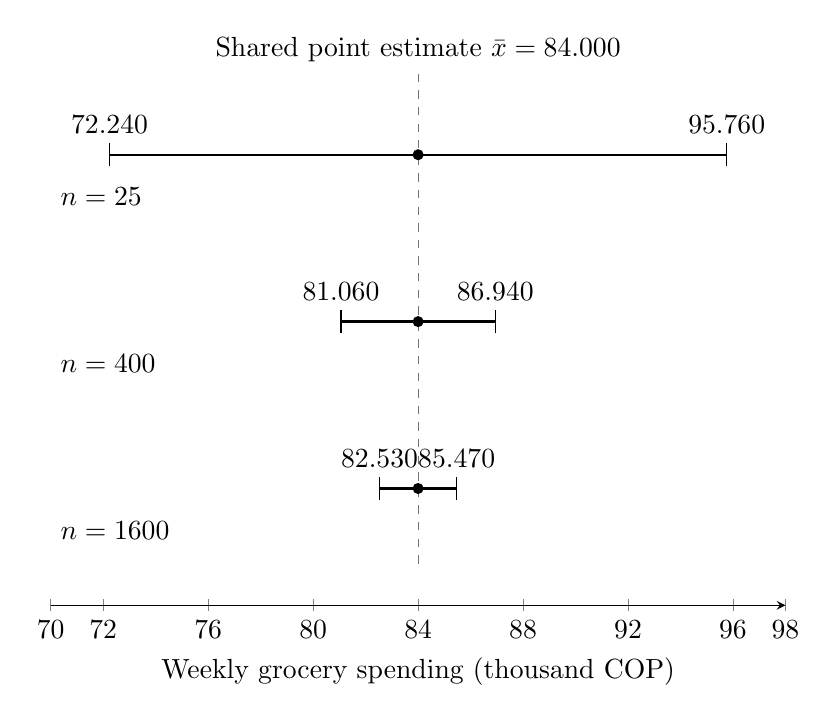
\begin{tikzpicture}\begin{axis}[
width=.9\linewidth,height=9cm,xmin=70,xmax=98,ymin=.3,ymax=3.8,
axis x line=bottom,axis y line=none,xtick={70,72,76,80,84,88,92,96,98},ytick=\empty,
xlabel={Weekly grocery spending (thousand COP)},scaled ticks=false,clip=false]
\draw[dashed,black!55] (axis cs:84,.55)--(axis cs:84,3.5);
\node[above] at (axis cs:84,3.5) {Shared point estimate $\bar{x}=84.000$};

\draw[thick] (axis cs:72.240,3)--(axis cs:95.760,3);
\draw (axis cs:72.240,3-.07)--(axis cs:72.240,3+.07)
(axis cs:95.760,3-.07)--(axis cs:95.760,3+.07);
\fill (axis cs:84,3) circle (2pt);
\node[above] at (axis cs:72.240,3+.07) {72.240};
\node[above] at (axis cs:95.760,3+.07) {95.760};
\node[anchor=west] at (axis cs:70,3-.25) {$n=25$};

\draw[thick] (axis cs:81.060,2)--(axis cs:86.940,2);
\draw (axis cs:81.060,2-.07)--(axis cs:81.060,2+.07)
(axis cs:86.940,2-.07)--(axis cs:86.940,2+.07);
\fill (axis cs:84,2) circle (2pt);
\node[above] at (axis cs:81.060,2+.07) {81.060};
\node[above] at (axis cs:86.940,2+.07) {86.940};
\node[anchor=west] at (axis cs:70,2-.25) {$n=400$};

\draw[thick] (axis cs:82.530,1)--(axis cs:85.470,1);
\draw (axis cs:82.530,1-.07)--(axis cs:82.530,1+.07)
(axis cs:85.470,1-.07)--(axis cs:85.470,1+.07);
\fill (axis cs:84,1) circle (2pt);
\node[above] at (axis cs:82.530,1+.07) {82.530};
\node[above] at (axis cs:85.470,1+.07) {85.470};
\node[anchor=west] at (axis cs:70,1-.25) {$n=1600$};
\end{axis}\end{tikzpicture}\end{center}
The same numerical scale and centre show the decreasing widths directly. Increasing sample size reduces sampling uncertainty and gives greater precision at the same nominal 95\% confidence.
\clearpage
\textbf{Problem 1 --- Weekly household grocery spending continued}
\task{Task 2:}{Illustrate the relationships between confidence level, critical value, and margin of error.}
Hold $n=100$ and $\sigma=30$ thousand COP fixed, so $\mathrm{SE}=\sigma/\sqrt n$ stays fixed. Assume a simple random sample of independent observations from a much larger population, known population SD, and a normal population or approximately normal sample mean.
Use $\mathrm{MoE}=z^*\times\mathrm{SE}$. Cases A--E are the five supplied pairs below; the ID stays the same across all three graphs. MoE uses thousand COP; $z^*$ is unitless and $C$ is a percentage.
\begin{datagrid}{|l|X|X|X|X|X|}ID&A&B&C&D&E\\\hline $C$ (\%)&80&90&95&99&99.9\\\hline $z^*$&1.282&1.645&1.960&2.576&3.291\\\hline\end{datagrid}
\textbf{Solution.} $\mathrm{SE}=30/\sqrt{100}=3.000$ thousand COP. Thus the five margins are $1.282(3)=3.846$, $1.645(3)=4.935$, $1.960(3)=5.880$, $2.576(3)=7.728$ and $3.291(3)=9.873$ thousand COP.
\par\smallskip
\begin{minipage}[t]{.49\linewidth}\vspace{0pt}\centering\textbf{Confidence level vs margin of error}\par\smallskip
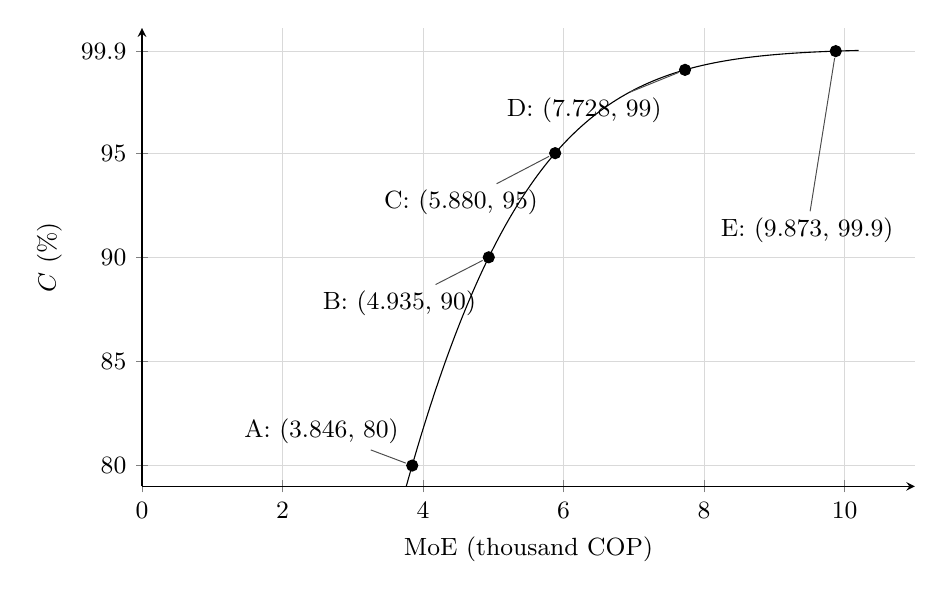
\begin{tikzpicture}\begin{axis}[relation,xlabel={MoE (thousand COP)},ylabel={$C$ (\%)},xmin=0,xmax=11,ymin=79,ymax=101,ytick={80,85,90,95,99.9}]
\addplot[black] coordinates {(3.600000000,76.986065956) (3.636666667,77.457267281) (3.673333333,77.921538814) (3.710000000,78.378914140) (3.746666667,78.829428390) (3.783333333,79.273118204) (3.820000000,79.710021689) (3.856666667,80.140178381) (3.893333333,80.563629207) (3.930000000,80.980416441) (3.966666667,81.390583669) (4.003333333,81.794175746) (4.040000000,82.191238757) (4.076666667,82.581819974) (4.113333333,82.965967820) (4.150000000,83.343731826) (4.186666667,83.715162592) (4.223333333,84.080311743) (4.260000000,84.439231895) (4.296666667,84.791976609) (4.333333333,85.138600354) (4.370000000,85.479158469) (4.406666667,85.813707116) (4.443333333,86.142303250) (4.480000000,86.465004571) (4.516666667,86.781869494) (4.553333333,87.092957100) (4.590000000,87.398327107) (4.626666667,87.698039826) (4.663333333,87.992156125) (4.700000000,88.280737392) (4.736666667,88.563845498) (4.773333333,88.841542760) (4.810000000,89.113891904) (4.846666667,89.380956033) (4.883333333,89.642798585) (4.920000000,89.899483305) (4.956666667,90.151074208) (4.993333333,90.397635545) (5.030000000,90.639231769) (5.066666667,90.875927504) (5.103333333,91.107787513) (5.140000000,91.334876665) (5.176666667,91.557259905) (5.213333333,91.775002224) (5.250000000,91.988168627) (5.286666667,92.196824108) (5.323333333,92.401033617) (5.360000000,92.600862035) (5.396666667,92.796374145) (5.433333333,92.987634608) (5.470000000,93.174707932) (5.506666667,93.357658453) (5.543333333,93.536550307) (5.580000000,93.711447404) (5.616666667,93.882413408) (5.653333333,94.049511715) (5.690000000,94.212805427) (5.726666667,94.372357332) (5.763333333,94.528229888) (5.800000000,94.680485196) (5.836666667,94.829184985) (5.873333333,94.974390591) (5.910000000,95.116162944) (5.946666667,95.254562542) (5.983333333,95.389649443) (6.020000000,95.521483244) (6.056666667,95.650123066) (6.093333333,95.775627542) (6.130000000,95.898054799) (6.166666667,96.017462450) (6.203333333,96.133907575) (6.240000000,96.247446713) (6.276666667,96.358135850) (6.313333333,96.466030405) (6.350000000,96.571185226) (6.386666667,96.673654573) (6.423333333,96.773492113) (6.460000000,96.870750912) (6.496666667,96.965483425) (6.533333333,97.057741490) (6.570000000,97.147576318) (6.606666667,97.235038493) (6.643333333,97.320177959) (6.680000000,97.403044022) (6.716666667,97.483685338) (6.753333333,97.562149914) (6.790000000,97.638485104) (6.826666667,97.712737601) (6.863333333,97.784953441) (6.900000000,97.855177996) (6.936666667,97.923455973) (6.973333333,97.989831414) (7.010000000,98.054347695) (7.046666667,98.117047523) (7.083333333,98.177972938) (7.120000000,98.237165314) (7.156666667,98.294665358) (7.193333333,98.350513110) (7.230000000,98.404747948) (7.266666667,98.457408586) (7.303333333,98.508533080) (7.340000000,98.558158826) (7.376666667,98.606322564) (7.413333333,98.653060386) (7.450000000,98.698407731) (7.486666667,98.742399394) (7.523333333,98.785069530) (7.560000000,98.826451657) (7.596666667,98.866578658) (7.633333333,98.905482789) (7.670000000,98.943195683) (7.706666667,98.979748356) (7.743333333,99.015171209) (7.780000000,99.049494036) (7.816666667,99.082746030) (7.853333333,99.114955789) (7.890000000,99.146151318) (7.926666667,99.176360042) (7.963333333,99.205608807) (8.000000000,99.233923886) (8.036666667,99.261330993) (8.073333333,99.287855279) (8.110000000,99.313521347) (8.146666667,99.338353257) (8.183333333,99.362374529) (8.220000000,99.385608156) (8.256666667,99.408076609) (8.293333333,99.429801841) (8.330000000,99.450805300) (8.366666667,99.471107932) (8.403333333,99.490730189) (8.440000000,99.509692041) (8.476666667,99.528012976) (8.513333333,99.545712013) (8.550000000,99.562807709) (8.586666667,99.579318164) (8.623333333,99.595261032) (8.660000000,99.610653524) (8.696666667,99.625512422) (8.733333333,99.639854079) (8.770000000,99.653694435) (8.806666667,99.667049015) (8.843333333,99.679932946) (8.880000000,99.692360958) (8.916666667,99.704347393) (8.953333333,99.715906214) (8.990000000,99.727051011) (9.026666667,99.737795010) (9.063333333,99.748151076) (9.100000000,99.758131727) (9.136666667,99.767749133) (9.173333333,99.777015132) (9.210000000,99.785941229) (9.246666667,99.794538609) (9.283333333,99.802818141) (9.320000000,99.810790383) (9.356666667,99.818465596) (9.393333333,99.825853741) (9.430000000,99.832964493) (9.466666667,99.839807245) (9.503333333,99.846391114) (9.540000000,99.852724948) (9.576666667,99.858817332) (9.613333333,99.864676596) (9.650000000,99.870310818) (9.686666667,99.875727832) (9.723333333,99.880935234) (9.760000000,99.885940387) (9.796666667,99.890750427) (9.833333333,99.895372271) (9.870000000,99.899812617) (9.906666667,99.904077957) (9.943333333,99.908174575) (9.980000000,99.912108558) (10.016666667,99.915885798) (10.053333333,99.919511999) (10.090000000,99.922992681) (10.126666667,99.926333183) (10.163333333,99.929538672) (10.200000000,99.932614147)};
\addplot[only marks,mark=*,mark size=2pt] coordinates {(3.846000000,80.000000000) (4.935000000,90.000000000) (5.880000000,95.000000000) (7.728000000,99.000000000) (9.873000000,99.900000000)};
\PointLabel{A}{3.846000000,80.000000000}{3.846}{80}{0.34}{0.12}{east}
\PointLabel{B}{4.935000000,90.000000000}{4.935}{90}{0.44}{0.4}{east}
\PointLabel{C}{5.880000000,95.000000000}{5.880}{95}{0.52}{0.62}{east}
\PointLabel{D}{7.728000000,99.000000000}{7.728}{99}{0.68}{0.82}{east}
\PointLabel{E}{9.873000000,99.900000000}{9.873}{99.9}{0.98}{0.56}{east}
\end{axis}\end{tikzpicture}\end{minipage}
\hfill
\begin{minipage}[t]{.49\linewidth}\vspace{0pt}\centering\textbf{Critical value vs margin of error}\par\smallskip
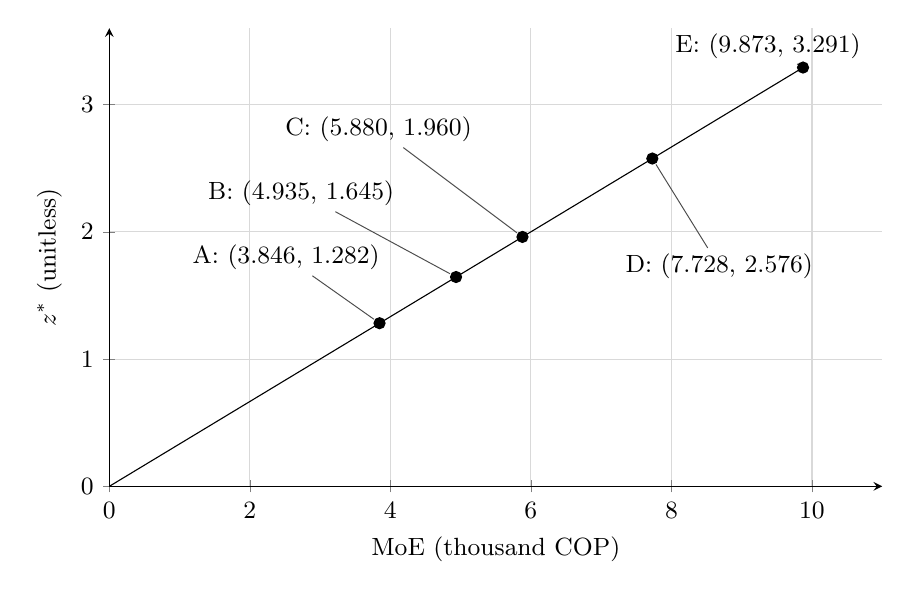
\begin{tikzpicture}\begin{axis}[relation,xlabel={MoE (thousand COP)},ylabel={$z^*$ (unitless)},xmin=0,xmax=11,ymin=0,ymax=3.6,ytick={0,1,2,3}]
\addplot[black,domain=0:9.873] {x/3.0};
\addplot[only marks,mark=*,mark size=2pt] coordinates {(3.846000000,1.282000000) (4.935000000,1.645000000) (5.880000000,1.960000000) (7.728000000,2.576000000) (9.873000000,3.291000000)};
\PointLabel{A}{3.846000000,1.282000000}{3.846}{1.282}{0.1}{0.5}{west}
\PointLabel{B}{4.935000000,1.645000000}{4.935}{1.645}{0.12}{0.64}{west}
\PointLabel{C}{5.880000000,1.960000000}{5.880}{1.960}{0.22}{0.78}{west}
\PointLabel{D}{7.728000000,2.576000000}{7.728}{2.576}{0.66}{0.48}{west}
\PointLabel{E}{9.873000000,3.291000000}{9.873}{3.291}{0.98}{0.96}{east}
\end{axis}\end{tikzpicture}\end{minipage}
\par\medskip
\begin{minipage}[t]{.49\linewidth}\vspace{0pt}\centering\textbf{Confidence level vs critical value}\par\smallskip
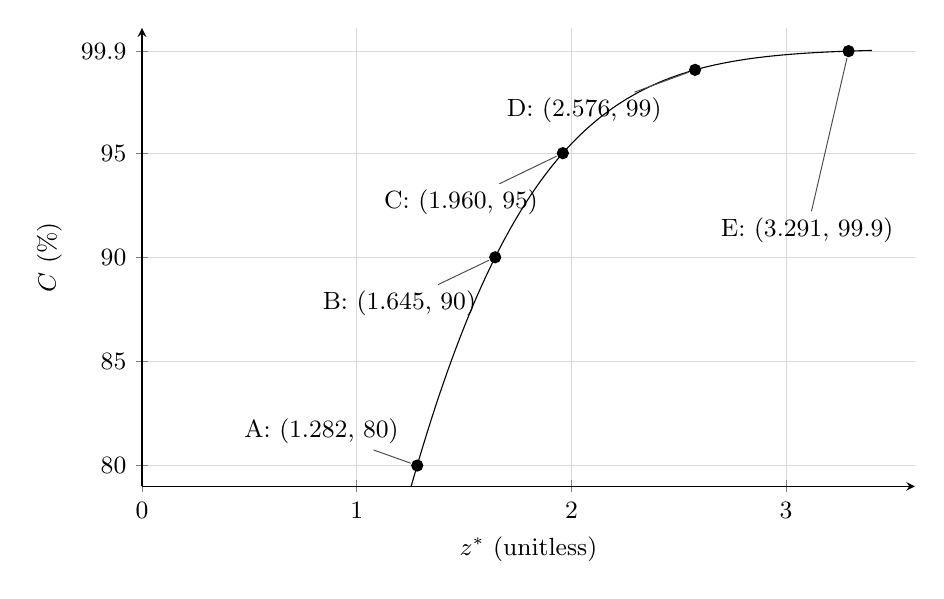
\begin{tikzpicture}\begin{axis}[relation,xlabel={$z^*$ (unitless)},ylabel={$C$ (\%)},xmin=0,xmax=3.6,ymin=79,ymax=101,xtick={0,1,2,3},ytick={80,85,90,95,99.9}]
\addplot[black] coordinates {(1.200000000,76.986065956) (1.212222222,77.457267281) (1.224444444,77.921538814) (1.236666667,78.378914140) (1.248888889,78.829428390) (1.261111111,79.273118204) (1.273333333,79.710021689) (1.285555556,80.140178381) (1.297777778,80.563629207) (1.310000000,80.980416441) (1.322222222,81.390583669) (1.334444444,81.794175746) (1.346666667,82.191238757) (1.358888889,82.581819974) (1.371111111,82.965967820) (1.383333333,83.343731826) (1.395555556,83.715162592) (1.407777778,84.080311743) (1.420000000,84.439231895) (1.432222222,84.791976609) (1.444444444,85.138600354) (1.456666667,85.479158469) (1.468888889,85.813707116) (1.481111111,86.142303250) (1.493333333,86.465004571) (1.505555556,86.781869494) (1.517777778,87.092957100) (1.530000000,87.398327107) (1.542222222,87.698039826) (1.554444444,87.992156125) (1.566666667,88.280737392) (1.578888889,88.563845498) (1.591111111,88.841542760) (1.603333333,89.113891904) (1.615555556,89.380956033) (1.627777778,89.642798585) (1.640000000,89.899483305) (1.652222222,90.151074208) (1.664444444,90.397635545) (1.676666667,90.639231769) (1.688888889,90.875927504) (1.701111111,91.107787513) (1.713333333,91.334876665) (1.725555556,91.557259905) (1.737777778,91.775002224) (1.750000000,91.988168627) (1.762222222,92.196824108) (1.774444444,92.401033617) (1.786666667,92.600862035) (1.798888889,92.796374145) (1.811111111,92.987634608) (1.823333333,93.174707932) (1.835555556,93.357658453) (1.847777778,93.536550307) (1.860000000,93.711447404) (1.872222222,93.882413408) (1.884444444,94.049511715) (1.896666667,94.212805427) (1.908888889,94.372357332) (1.921111111,94.528229888) (1.933333333,94.680485196) (1.945555556,94.829184985) (1.957777778,94.974390591) (1.970000000,95.116162944) (1.982222222,95.254562542) (1.994444444,95.389649443) (2.006666667,95.521483244) (2.018888889,95.650123066) (2.031111111,95.775627542) (2.043333333,95.898054799) (2.055555556,96.017462450) (2.067777778,96.133907575) (2.080000000,96.247446713) (2.092222222,96.358135850) (2.104444444,96.466030405) (2.116666667,96.571185226) (2.128888889,96.673654573) (2.141111111,96.773492113) (2.153333333,96.870750912) (2.165555556,96.965483425) (2.177777778,97.057741490) (2.190000000,97.147576318) (2.202222222,97.235038493) (2.214444444,97.320177959) (2.226666667,97.403044022) (2.238888889,97.483685338) (2.251111111,97.562149914) (2.263333333,97.638485104) (2.275555556,97.712737601) (2.287777778,97.784953441) (2.300000000,97.855177996) (2.312222222,97.923455973) (2.324444444,97.989831414) (2.336666667,98.054347695) (2.348888889,98.117047523) (2.361111111,98.177972938) (2.373333333,98.237165314) (2.385555556,98.294665358) (2.397777778,98.350513110) (2.410000000,98.404747948) (2.422222222,98.457408586) (2.434444444,98.508533080) (2.446666667,98.558158826) (2.458888889,98.606322564) (2.471111111,98.653060386) (2.483333333,98.698407731) (2.495555556,98.742399394) (2.507777778,98.785069530) (2.520000000,98.826451657) (2.532222222,98.866578658) (2.544444444,98.905482789) (2.556666667,98.943195683) (2.568888889,98.979748356) (2.581111111,99.015171209) (2.593333333,99.049494036) (2.605555556,99.082746030) (2.617777778,99.114955789) (2.630000000,99.146151318) (2.642222222,99.176360042) (2.654444444,99.205608807) (2.666666667,99.233923886) (2.678888889,99.261330993) (2.691111111,99.287855279) (2.703333333,99.313521347) (2.715555556,99.338353257) (2.727777778,99.362374529) (2.740000000,99.385608156) (2.752222222,99.408076609) (2.764444444,99.429801841) (2.776666667,99.450805300) (2.788888889,99.471107932) (2.801111111,99.490730189) (2.813333333,99.509692041) (2.825555556,99.528012976) (2.837777778,99.545712013) (2.850000000,99.562807709) (2.862222222,99.579318164) (2.874444444,99.595261032) (2.886666667,99.610653524) (2.898888889,99.625512422) (2.911111111,99.639854079) (2.923333333,99.653694435) (2.935555556,99.667049015) (2.947777778,99.679932946) (2.960000000,99.692360958) (2.972222222,99.704347393) (2.984444444,99.715906214) (2.996666667,99.727051011) (3.008888889,99.737795010) (3.021111111,99.748151076) (3.033333333,99.758131727) (3.045555556,99.767749133) (3.057777778,99.777015132) (3.070000000,99.785941229) (3.082222222,99.794538609) (3.094444444,99.802818141) (3.106666667,99.810790383) (3.118888889,99.818465596) (3.131111111,99.825853741) (3.143333333,99.832964493) (3.155555556,99.839807245) (3.167777778,99.846391114) (3.180000000,99.852724948) (3.192222222,99.858817332) (3.204444444,99.864676596) (3.216666667,99.870310818) (3.228888889,99.875727832) (3.241111111,99.880935234) (3.253333333,99.885940387) (3.265555556,99.890750427) (3.277777778,99.895372271) (3.290000000,99.899812617) (3.302222222,99.904077957) (3.314444444,99.908174575) (3.326666667,99.912108558) (3.338888889,99.915885798) (3.351111111,99.919511999) (3.363333333,99.922992681) (3.375555556,99.926333183) (3.387777778,99.929538672) (3.400000000,99.932614147)};
\addplot[only marks,mark=*,mark size=2pt] coordinates {(1.282000000,80.000000000) (1.645000000,90.000000000) (1.960000000,95.000000000) (2.576000000,99.000000000) (3.291000000,99.900000000)};
\PointLabel{A}{1.282000000,80.000000000}{1.282}{80}{0.34}{0.12}{east}
\PointLabel{B}{1.645000000,90.000000000}{1.645}{90}{0.44}{0.4}{east}
\PointLabel{C}{1.960000000,95.000000000}{1.960}{95}{0.52}{0.62}{east}
\PointLabel{D}{2.576000000,99.000000000}{2.576}{99}{0.68}{0.82}{east}
\PointLabel{E}{3.291000000,99.900000000}{3.291}{99.9}{0.98}{0.56}{east}
\end{axis}\end{tikzpicture}\end{minipage}
\par\clearpage
\textbf{Problem 1 --- Task 2 solution continued}\par
At fixed SE, $z^*=\mathrm{MoE}/3$ is a line through the origin. Higher confidence requires a larger cutoff and margin, while SE stays unchanged.
The smooth confidence curves use $100[2\Phi(z^*)-1]$, or $100[2\Phi(\mathrm{MoE}/3)-1]$, where $\Phi$ is the standard normal CDF. The five points use the nominal supplied percentages. Rounding the cutoffs causes a very small difference between these points and the theoretical curves.

\textbf{Explanatory standard normal illustrations}\par
The panels correspond to cases A, C and E of Task 2. Each uses the same horizontal scale $-4\le z\le4$ and density scale $0\le f(z)\le0.46$.
\par\bigskip
\normalpanel{80}{1.282}\hfill\normalpanel{95}{1.960}\hfill\normalpanel{99.9}{3.291}
\par\bigskip
Each shaded central region is bounded by $-z^*$ and $+z^*$. The central labels give nominal confidence; the rounded cutoffs enclose approximately 80.01574\%, 95.00042\% and 99.90017\%, respectively.
As confidence increases, the cutoffs move outward under the same curve. The larger margin gives a wider interval around the same point estimate: nominal long-run coverage rises while precision decreases.
\clearpage
\stageheading{Guided Example}
\problemtitle{2}{Delivery charges for local businesses}
A business association estimates the mean charge for a local delivery.
\task{Task 1:}{Illustrate the relationships between standard error, margin of error, and sample size.}
Hold $\sigma=24$ thousand COP and $C=95\%$ ($z^*=1.960$) fixed. Assume a simple random sample of independent observations from a much larger population, known population SD, and a normal population or approximately normal sample mean.
Use $\mathrm{SE}=\sigma/\sqrt n$ and $\mathrm{MoE}=z^*\times\mathrm{SE}$. Cases A--E correspond, in order, to $n=36,100,225,400,900$. Each of the three graphs uses these five cases and five coordinate labels. SE and MoE use thousand COP.
Complete the three relationship graphs, each with five plotted points, their coordinate labels, and the relationship curve. Keep each ID attached to the same case. Retain unrounded intermediate values; write calculated coordinates to three decimals. The workspace is for calculations within this task.
\par\smallskip
\begin{minipage}[t]{.49\linewidth}\vspace{0pt}\centering\textbf{Standard error vs sample size}\par\smallskip
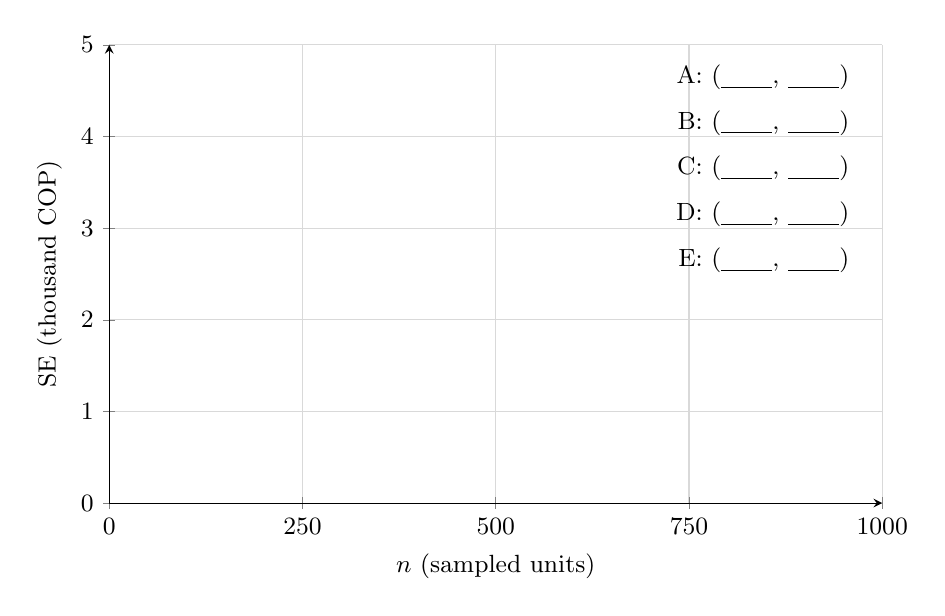
\begin{tikzpicture}\begin{axis}[relation,xlabel={$n$ (sampled units)},ylabel={SE (thousand COP)},xmin=0,xmax=1000,ymin=0,ymax=5,xtick={0,250,500,750,1000}]
\LabelTemplates
\end{axis}\end{tikzpicture}\end{minipage}
\hfill
\begin{minipage}[t]{.49\linewidth}\vspace{0pt}\centering\textbf{Margin of error vs sample size}\par\smallskip
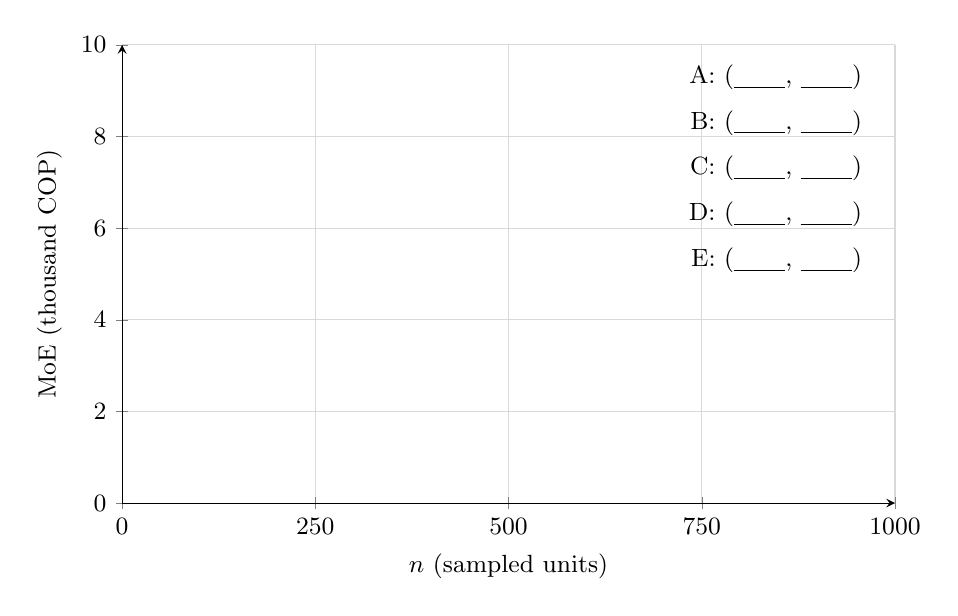
\begin{tikzpicture}\begin{axis}[relation,xlabel={$n$ (sampled units)},ylabel={MoE (thousand COP)},xmin=0,xmax=1000,ymin=0,ymax=10,xtick={0,250,500,750,1000}]
\LabelTemplates
\end{axis}\end{tikzpicture}\end{minipage}
\par\medskip
\begin{minipage}[t]{.49\linewidth}\vspace{0pt}\centering\textbf{Margin of error vs standard error}\par\smallskip
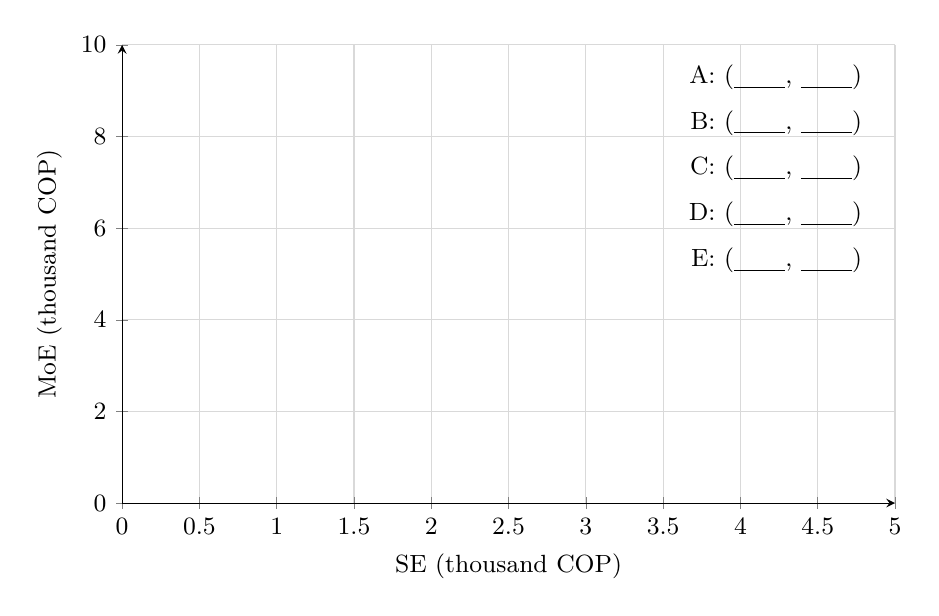
\begin{tikzpicture}\begin{axis}[relation,xlabel={SE (thousand COP)},ylabel={MoE (thousand COP)},xmin=0,xmax=5,ymin=0,ymax=10]
\LabelTemplates
\end{axis}\end{tikzpicture}\end{minipage}
\hfill\workarea\par
\clearpage
\textbf{Problem 2 --- Delivery charges for local businesses continued}
\task{Task 2:}{Illustrate the relationships between confidence level, critical value, and margin of error.}
Hold $n=100$ and $\sigma=24$ thousand COP fixed, so $\mathrm{SE}=\sigma/\sqrt n$ stays fixed. Assume a simple random sample of independent observations from a much larger population, known population SD, and a normal population or approximately normal sample mean.
Use $\mathrm{MoE}=z^*\times\mathrm{SE}$. Cases A--E are the five supplied pairs below; the ID stays the same across all three graphs. MoE uses thousand COP; $z^*$ is unitless and $C$ is a percentage.
\begin{datagrid}{|l|X|X|X|X|X|}ID&A&B&C&D&E\\\hline $C$ (\%)&80&90&95&99&99.9\\\hline $z^*$&1.282&1.645&1.960&2.576&3.291\\\hline\end{datagrid}
Complete the three relationship graphs with five labeled points and the relationship curves. Use true numerical spacing, including near 100\%. Retain unrounded intermediate values; write calculated coordinates to three decimals. The workspace is for calculations within this task.
\par\smallskip
\begin{minipage}[t]{.49\linewidth}\vspace{0pt}\centering\textbf{Confidence level vs margin of error}\par\smallskip
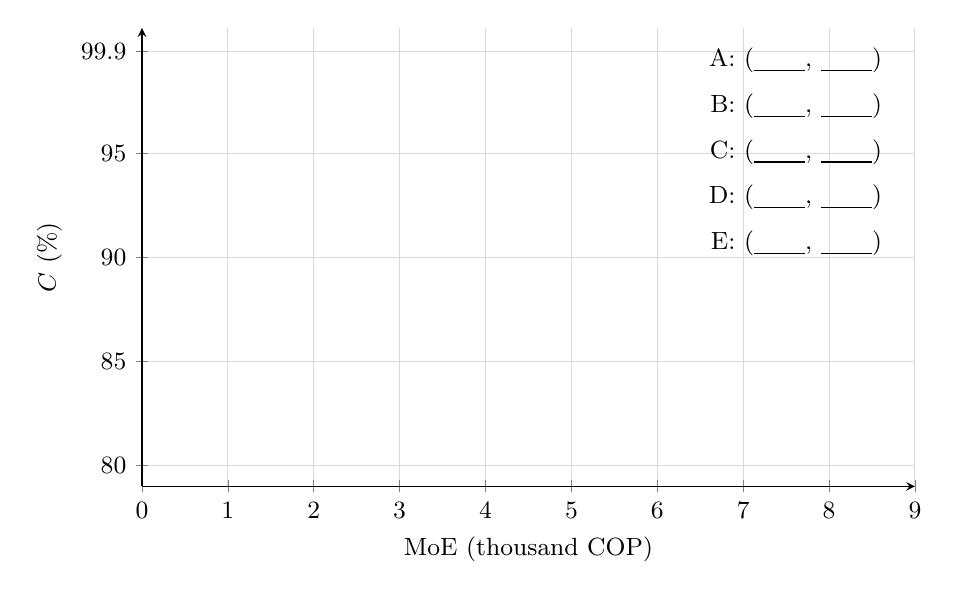
\begin{tikzpicture}\begin{axis}[relation,xlabel={MoE (thousand COP)},ylabel={$C$ (\%)},xmin=0,xmax=9,ymin=79,ymax=101,ytick={80,85,90,95,99.9}]
\LabelTemplates
\end{axis}\end{tikzpicture}\end{minipage}
\hfill
\begin{minipage}[t]{.49\linewidth}\vspace{0pt}\centering\textbf{Critical value vs margin of error}\par\smallskip
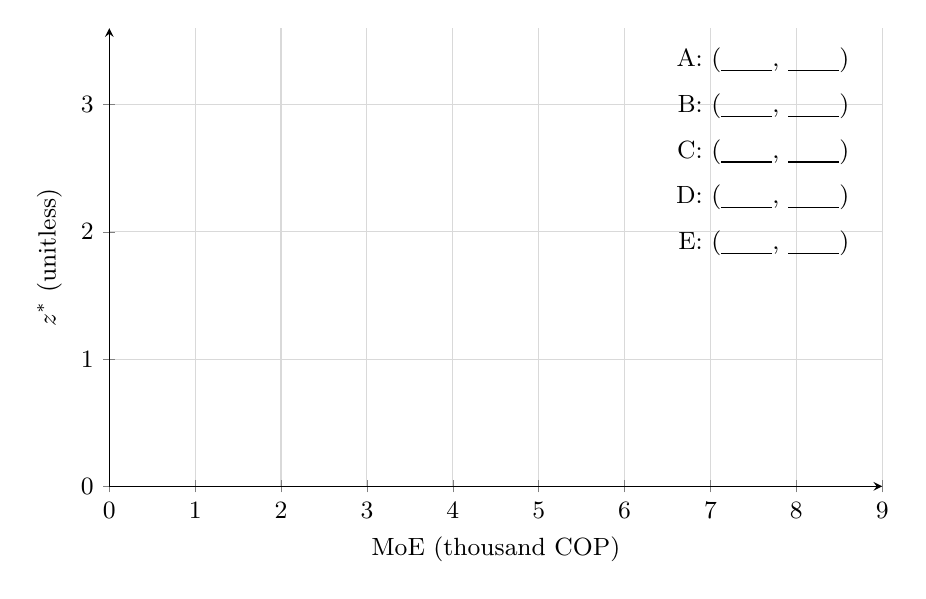
\begin{tikzpicture}\begin{axis}[relation,xlabel={MoE (thousand COP)},ylabel={$z^*$ (unitless)},xmin=0,xmax=9,ymin=0,ymax=3.6,ytick={0,1,2,3}]
\LabelTemplates
\end{axis}\end{tikzpicture}\end{minipage}
\par\medskip
\begin{minipage}[t]{.49\linewidth}\vspace{0pt}\centering\textbf{Confidence level vs critical value}\par\smallskip
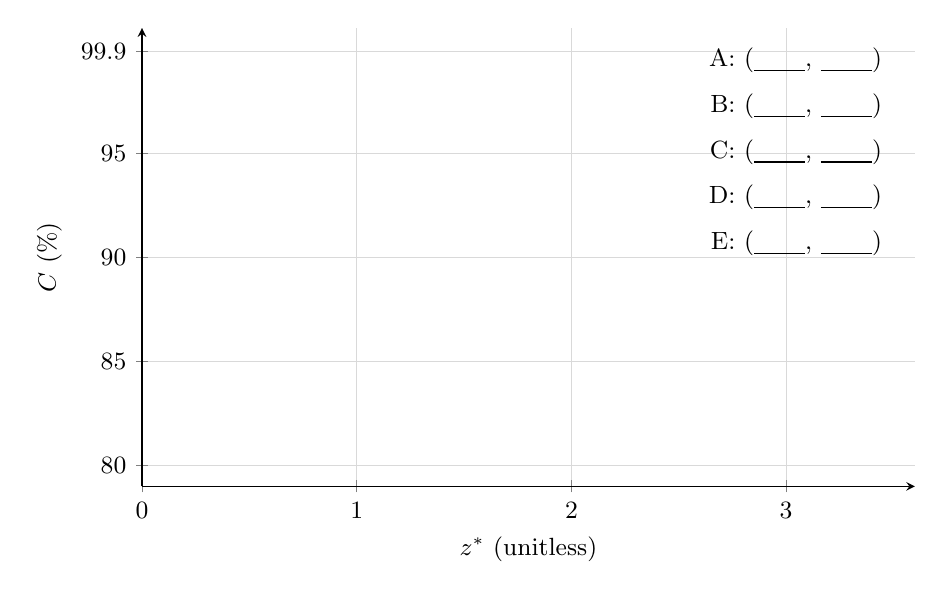
\begin{tikzpicture}\begin{axis}[relation,xlabel={$z^*$ (unitless)},ylabel={$C$ (\%)},xmin=0,xmax=3.6,ymin=79,ymax=101,xtick={0,1,2,3},ytick={80,85,90,95,99.9}]
\LabelTemplates
\end{axis}\end{tikzpicture}\end{minipage}
\hfill\workarea\par
\clearpage
\stageheading{Independent Practice}
\problemtitle{3}{Weekly market-stall revenue}
A market office estimates mean weekly revenue per stall.
\task{Task 1:}{Illustrate the relationships between standard error, margin of error, and sample size.}
Hold $\sigma=45$ thousand COP and $C=95\%$ ($z^*=1.960$) fixed. Assume a simple random sample of independent observations from a much larger population, known population SD, and a normal population or approximately normal sample mean.
Use $\mathrm{SE}=\sigma/\sqrt n$ and $\mathrm{MoE}=z^*\times\mathrm{SE}$. Cases A--E correspond, in order, to $n=25,100,225,625,1600$. Each of the three graphs uses these five cases and five coordinate labels. SE and MoE use thousand COP.
Complete the three relationship graphs, each with five plotted points, their coordinate labels, and the relationship curve. Keep each ID attached to the same case. Retain unrounded intermediate values; write calculated coordinates to three decimals. The workspace is for calculations within this task.
\par\smallskip
\begin{minipage}[t]{.49\linewidth}\vspace{0pt}\centering\textbf{Standard error vs sample size}\par\smallskip
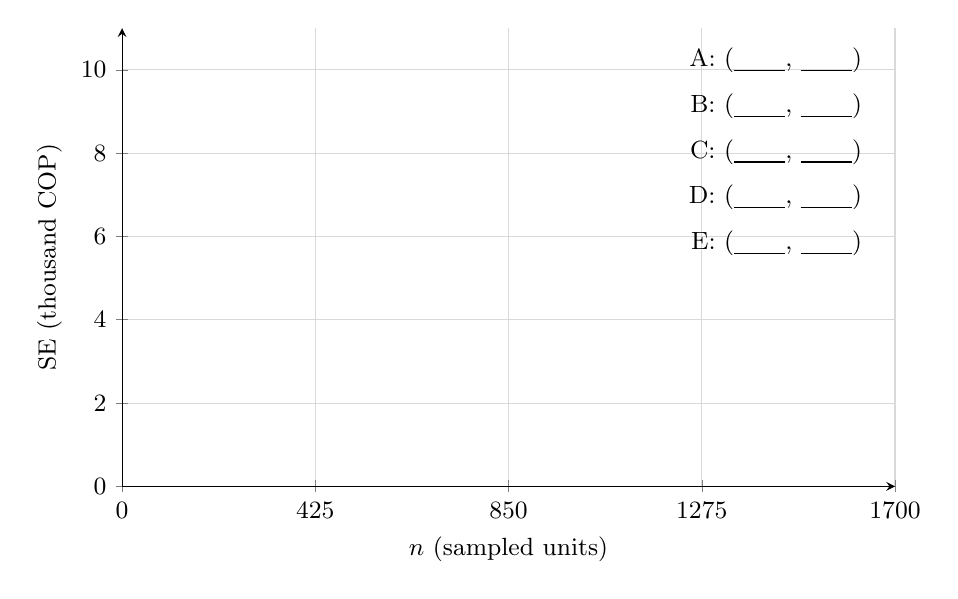
\begin{tikzpicture}\begin{axis}[relation,xlabel={$n$ (sampled units)},ylabel={SE (thousand COP)},xmin=0,xmax=1700,ymin=0,ymax=11,xtick={0,425,850,1275,1700}]
\LabelTemplates
\end{axis}\end{tikzpicture}\end{minipage}
\hfill
\begin{minipage}[t]{.49\linewidth}\vspace{0pt}\centering\textbf{Margin of error vs sample size}\par\smallskip
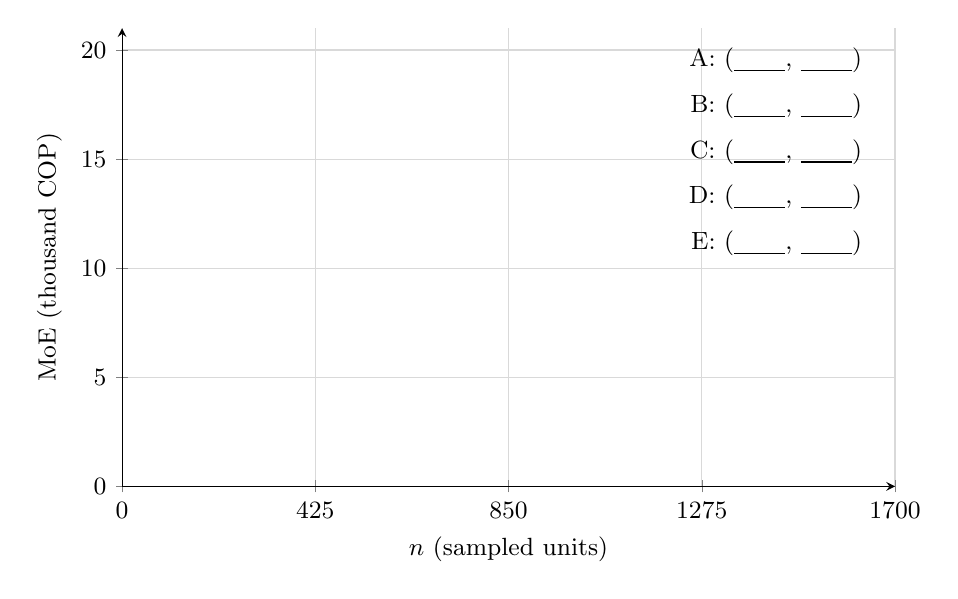
\begin{tikzpicture}\begin{axis}[relation,xlabel={$n$ (sampled units)},ylabel={MoE (thousand COP)},xmin=0,xmax=1700,ymin=0,ymax=21,xtick={0,425,850,1275,1700}]
\LabelTemplates
\end{axis}\end{tikzpicture}\end{minipage}
\par\medskip
\begin{minipage}[t]{.49\linewidth}\vspace{0pt}\centering\textbf{Margin of error vs standard error}\par\smallskip
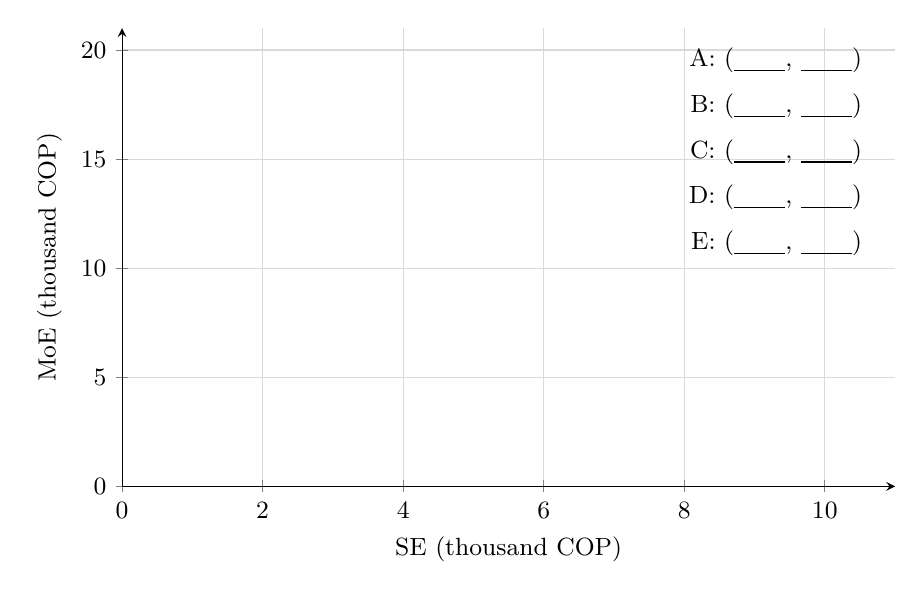
\begin{tikzpicture}\begin{axis}[relation,xlabel={SE (thousand COP)},ylabel={MoE (thousand COP)},xmin=0,xmax=11,ymin=0,ymax=21]
\LabelTemplates
\end{axis}\end{tikzpicture}\end{minipage}
\hfill\workarea\par
\clearpage
\textbf{Problem 3 --- Weekly market-stall revenue continued}
\task{Task 2:}{Illustrate the relationships between confidence level, critical value, and margin of error.}
Hold $n=225$ and $\sigma=45$ thousand COP fixed, so $\mathrm{SE}=\sigma/\sqrt n$ stays fixed. Assume a simple random sample of independent observations from a much larger population, known population SD, and a normal population or approximately normal sample mean.
Use $\mathrm{MoE}=z^*\times\mathrm{SE}$. Cases A--E are the five supplied pairs below; the ID stays the same across all three graphs. MoE uses thousand COP; $z^*$ is unitless and $C$ is a percentage.
\begin{datagrid}{|l|X|X|X|X|X|}ID&A&B&C&D&E\\\hline $C$ (\%)&80&90&95&99&99.9\\\hline $z^*$&1.282&1.645&1.960&2.576&3.291\\\hline\end{datagrid}
Complete the three relationship graphs with five labeled points and the relationship curves. Use true numerical spacing, including near 100\%. Retain unrounded intermediate values; write calculated coordinates to three decimals. The workspace is for calculations within this task.
\par\smallskip
\begin{minipage}[t]{.49\linewidth}\vspace{0pt}\centering\textbf{Confidence level vs margin of error}\par\smallskip
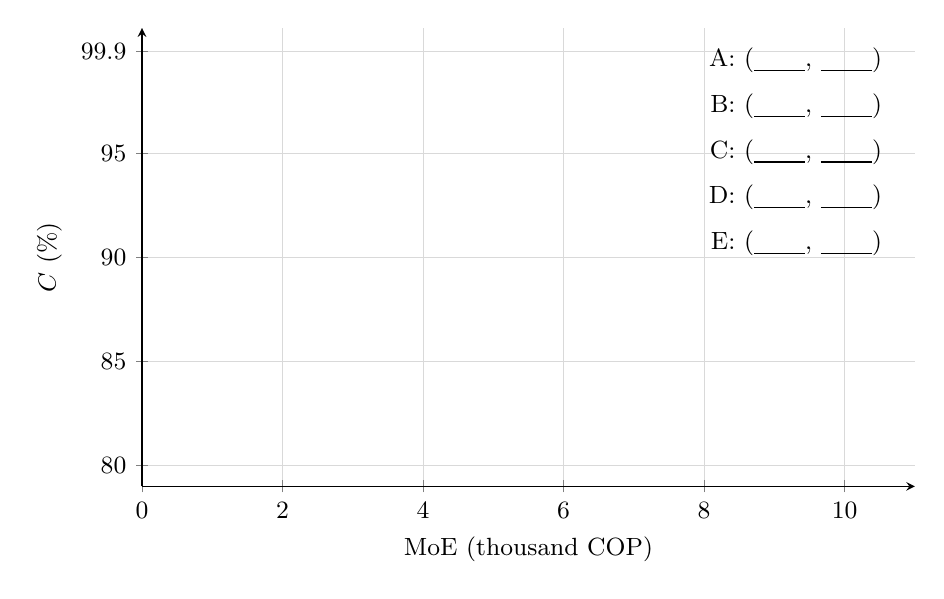
\begin{tikzpicture}\begin{axis}[relation,xlabel={MoE (thousand COP)},ylabel={$C$ (\%)},xmin=0,xmax=11,ymin=79,ymax=101,ytick={80,85,90,95,99.9}]
\LabelTemplates
\end{axis}\end{tikzpicture}\end{minipage}
\hfill
\begin{minipage}[t]{.49\linewidth}\vspace{0pt}\centering\textbf{Critical value vs margin of error}\par\smallskip
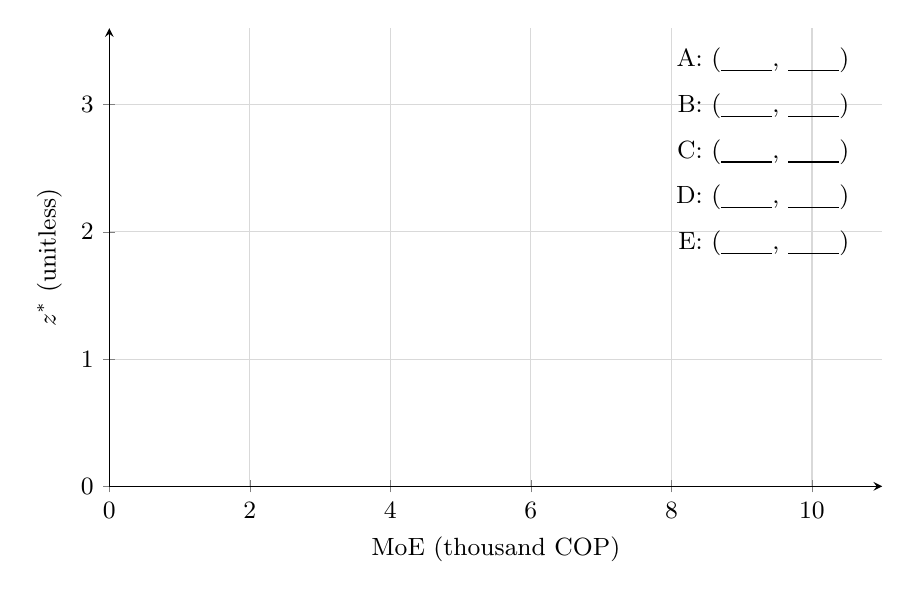
\begin{tikzpicture}\begin{axis}[relation,xlabel={MoE (thousand COP)},ylabel={$z^*$ (unitless)},xmin=0,xmax=11,ymin=0,ymax=3.6,ytick={0,1,2,3}]
\LabelTemplates
\end{axis}\end{tikzpicture}\end{minipage}
\par\medskip
\begin{minipage}[t]{.49\linewidth}\vspace{0pt}\centering\textbf{Confidence level vs critical value}\par\smallskip
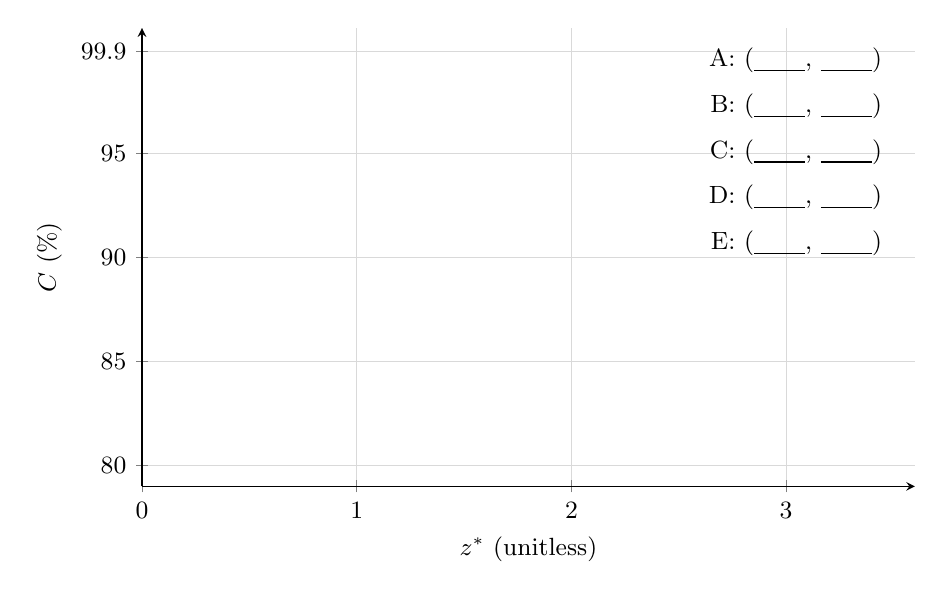
\begin{tikzpicture}\begin{axis}[relation,xlabel={$z^*$ (unitless)},ylabel={$C$ (\%)},xmin=0,xmax=3.6,ymin=79,ymax=101,xtick={0,1,2,3},ytick={80,85,90,95,99.9}]
\LabelTemplates
\end{axis}\end{tikzpicture}\end{minipage}
\hfill\workarea\par
\clearpage
\problemtitle{4}{Freight handling fees}
A port analyst estimates the mean handling fee per container.
\task{Task 1:}{Illustrate the relationships between standard error, margin of error, and sample size.}
Hold $\sigma=72$ USD and $C=95\%$ ($z^*=1.960$) fixed. Assume a simple random sample of independent observations from a much larger population, known population SD, and a normal population or approximately normal sample mean.
Use $\mathrm{SE}=\sigma/\sqrt n$ and $\mathrm{MoE}=z^*\times\mathrm{SE}$. Cases A--E correspond, in order, to $n=36,144,324,576,1296$. Each of the three graphs uses these five cases and five coordinate labels. SE and MoE use USD.
Complete the three relationship graphs, each with five plotted points, their coordinate labels, and the relationship curve. Keep each ID attached to the same case. Retain unrounded intermediate values; write calculated coordinates to three decimals. The workspace is for calculations within this task.
\par\smallskip
\begin{minipage}[t]{.49\linewidth}\vspace{0pt}\centering\textbf{Standard error vs sample size}\par\smallskip
\begin{tikzpicture}\begin{axis}[relation,xlabel={$n$ (sampled units)},ylabel={SE (USD)},xmin=0,xmax=1400,ymin=0,ymax=14,xtick={0,350,700,1050,1400}]
\LabelTemplates
\end{axis}\end{tikzpicture}\end{minipage}
\hfill
\begin{minipage}[t]{.49\linewidth}\vspace{0pt}\centering\textbf{Margin of error vs sample size}\par\smallskip
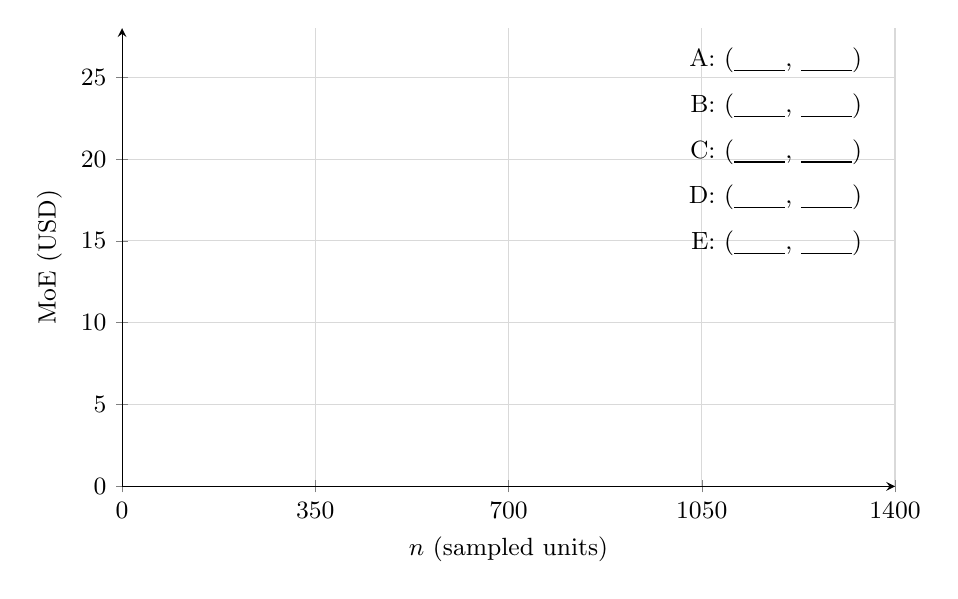
\begin{tikzpicture}\begin{axis}[relation,xlabel={$n$ (sampled units)},ylabel={MoE (USD)},xmin=0,xmax=1400,ymin=0,ymax=28,xtick={0,350,700,1050,1400}]
\LabelTemplates
\end{axis}\end{tikzpicture}\end{minipage}
\par\medskip
\begin{minipage}[t]{.49\linewidth}\vspace{0pt}\centering\textbf{Margin of error vs standard error}\par\smallskip
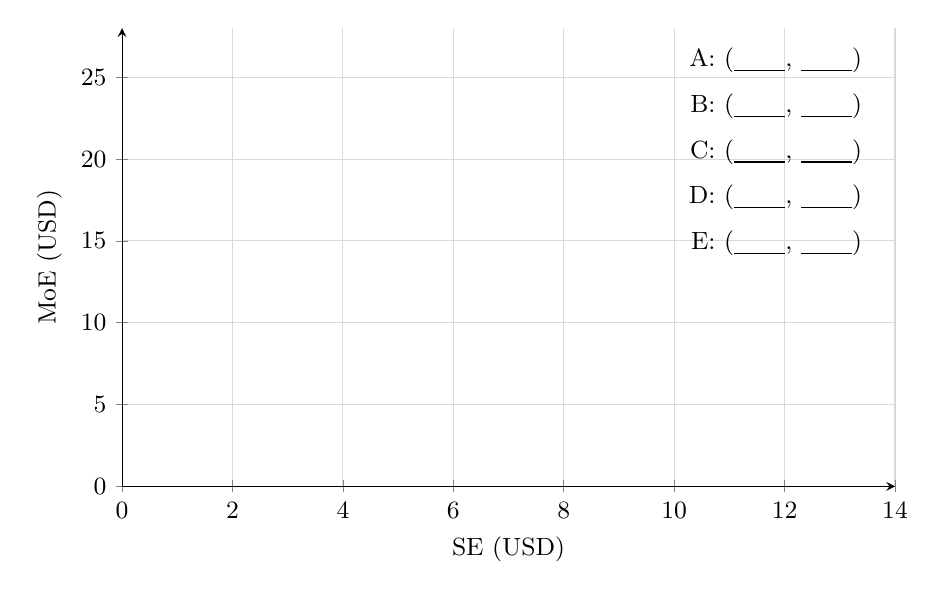
\begin{tikzpicture}\begin{axis}[relation,xlabel={SE (USD)},ylabel={MoE (USD)},xmin=0,xmax=14,ymin=0,ymax=28]
\LabelTemplates
\end{axis}\end{tikzpicture}\end{minipage}
\hfill\workarea\par
\clearpage
\textbf{Problem 4 --- Freight handling fees continued}
\task{Task 2:}{Illustrate the relationships between confidence level, critical value, and margin of error.}
Hold $n=144$ and $\sigma=72$ USD fixed, so $\mathrm{SE}=\sigma/\sqrt n$ stays fixed. Assume a simple random sample of independent observations from a much larger population, known population SD, and a normal population or approximately normal sample mean.
Use $\mathrm{MoE}=z^*\times\mathrm{SE}$. Cases A--E are the five supplied pairs below; the ID stays the same across all three graphs. MoE uses USD; $z^*$ is unitless and $C$ is a percentage.
\begin{datagrid}{|l|X|X|X|X|X|}ID&A&B&C&D&E\\\hline $C$ (\%)&80&90&95&99&99.9\\\hline $z^*$&1.282&1.645&1.960&2.576&3.291\\\hline\end{datagrid}
Complete the three relationship graphs with five labeled points and the relationship curves. Use true numerical spacing, including near 100\%. Retain unrounded intermediate values; write calculated coordinates to three decimals. The workspace is for calculations within this task.
\par\smallskip
\begin{minipage}[t]{.49\linewidth}\vspace{0pt}\centering\textbf{Confidence level vs margin of error}\par\smallskip
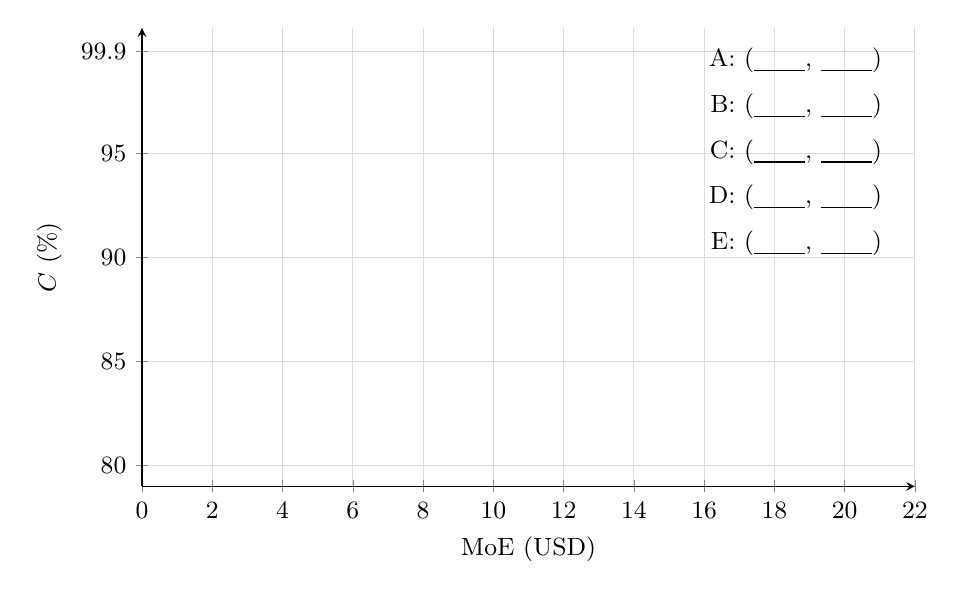
\begin{tikzpicture}\begin{axis}[relation,xlabel={MoE (USD)},ylabel={$C$ (\%)},xmin=0,xmax=22,ymin=79,ymax=101,ytick={80,85,90,95,99.9}]
\LabelTemplates
\end{axis}\end{tikzpicture}\end{minipage}
\hfill
\begin{minipage}[t]{.49\linewidth}\vspace{0pt}\centering\textbf{Critical value vs margin of error}\par\smallskip
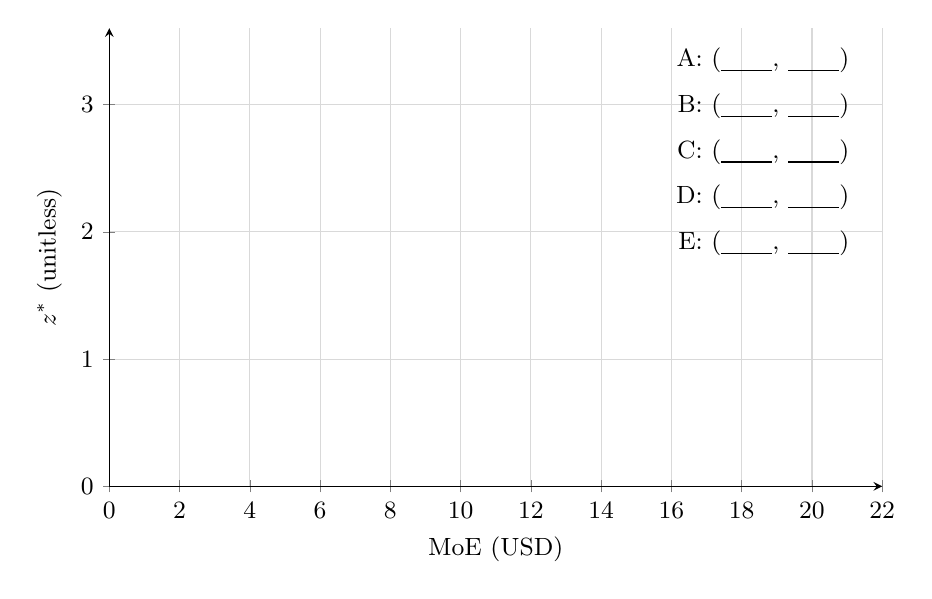
\begin{tikzpicture}\begin{axis}[relation,xlabel={MoE (USD)},ylabel={$z^*$ (unitless)},xmin=0,xmax=22,ymin=0,ymax=3.6,ytick={0,1,2,3}]
\LabelTemplates
\end{axis}\end{tikzpicture}\end{minipage}
\par\medskip
\begin{minipage}[t]{.49\linewidth}\vspace{0pt}\centering\textbf{Confidence level vs critical value}\par\smallskip
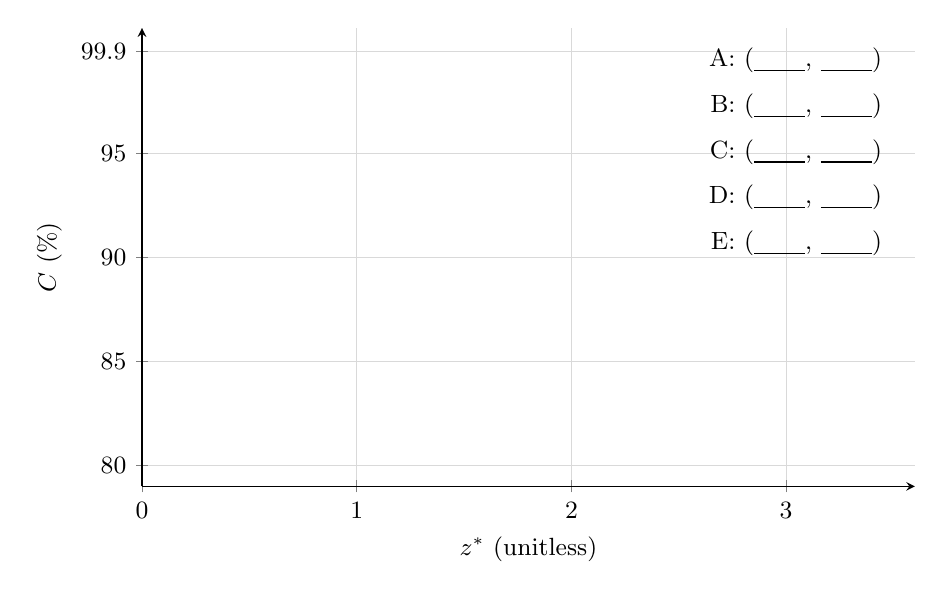
\begin{tikzpicture}\begin{axis}[relation,xlabel={$z^*$ (unitless)},ylabel={$C$ (\%)},xmin=0,xmax=3.6,ymin=79,ymax=101,xtick={0,1,2,3},ytick={80,85,90,95,99.9}]
\LabelTemplates
\end{axis}\end{tikzpicture}\end{minipage}
\hfill\workarea\par
\clearpage
\problemtitle{5}{Monthly internet costs}
A district estimates mean monthly internet expenditure per small business.
\task{Task 1:}{Illustrate the relationships between standard error, margin of error, and sample size.}
Hold $\sigma=35$ thousand COP and $C=95\%$ ($z^*=1.960$) fixed. Assume a simple random sample of independent observations from a much larger population, known population SD, and a normal population or approximately normal sample mean.
Use $\mathrm{SE}=\sigma/\sqrt n$ and $\mathrm{MoE}=z^*\times\mathrm{SE}$. Cases A--E correspond, in order, to $n=49,100,196,400,1225$. Each of the three graphs uses these five cases and five coordinate labels. SE and MoE use thousand COP.
Complete the three relationship graphs, each with five plotted points, their coordinate labels, and the relationship curve. Keep each ID attached to the same case. Retain unrounded intermediate values; write calculated coordinates to three decimals. The workspace is for calculations within this task.
\par\smallskip
\begin{minipage}[t]{.49\linewidth}\vspace{0pt}\centering\textbf{Standard error vs sample size}\par\smallskip
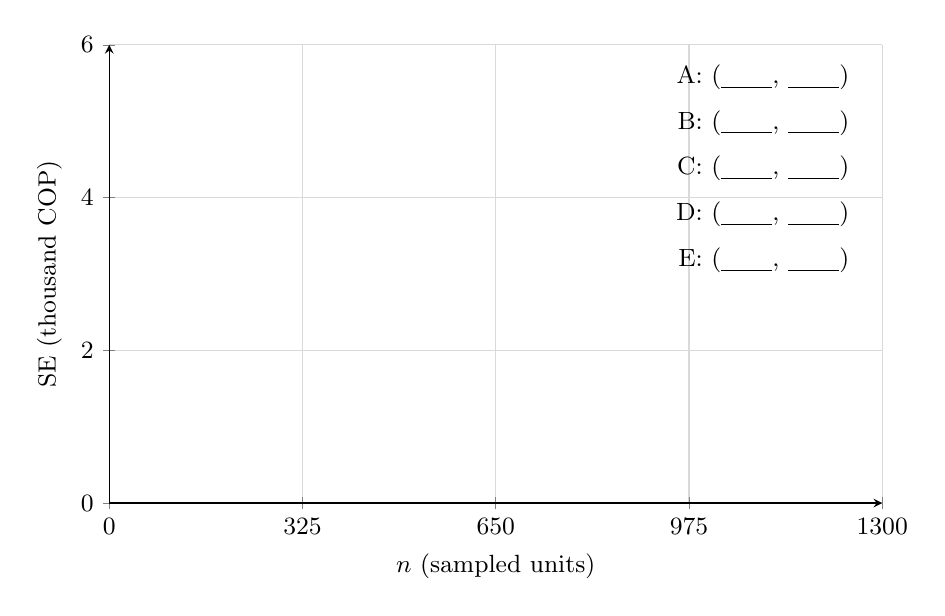
\begin{tikzpicture}\begin{axis}[relation,xlabel={$n$ (sampled units)},ylabel={SE (thousand COP)},xmin=0,xmax=1300,ymin=0,ymax=6,xtick={0,325,650,975,1300}]
\LabelTemplates
\end{axis}\end{tikzpicture}\end{minipage}
\hfill
\begin{minipage}[t]{.49\linewidth}\vspace{0pt}\centering\textbf{Margin of error vs sample size}\par\smallskip
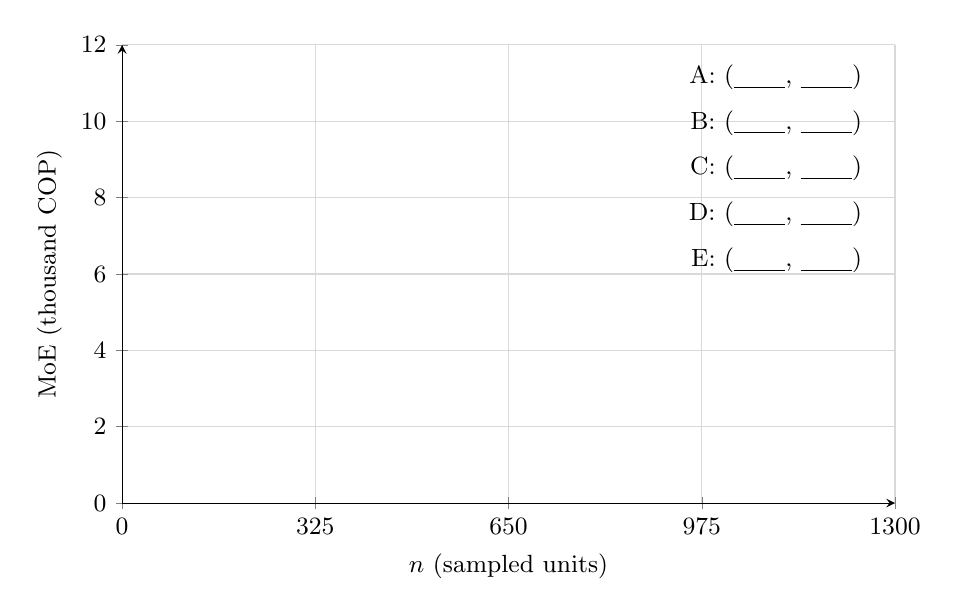
\begin{tikzpicture}\begin{axis}[relation,xlabel={$n$ (sampled units)},ylabel={MoE (thousand COP)},xmin=0,xmax=1300,ymin=0,ymax=12,xtick={0,325,650,975,1300}]
\LabelTemplates
\end{axis}\end{tikzpicture}\end{minipage}
\par\medskip
\begin{minipage}[t]{.49\linewidth}\vspace{0pt}\centering\textbf{Margin of error vs standard error}\par\smallskip
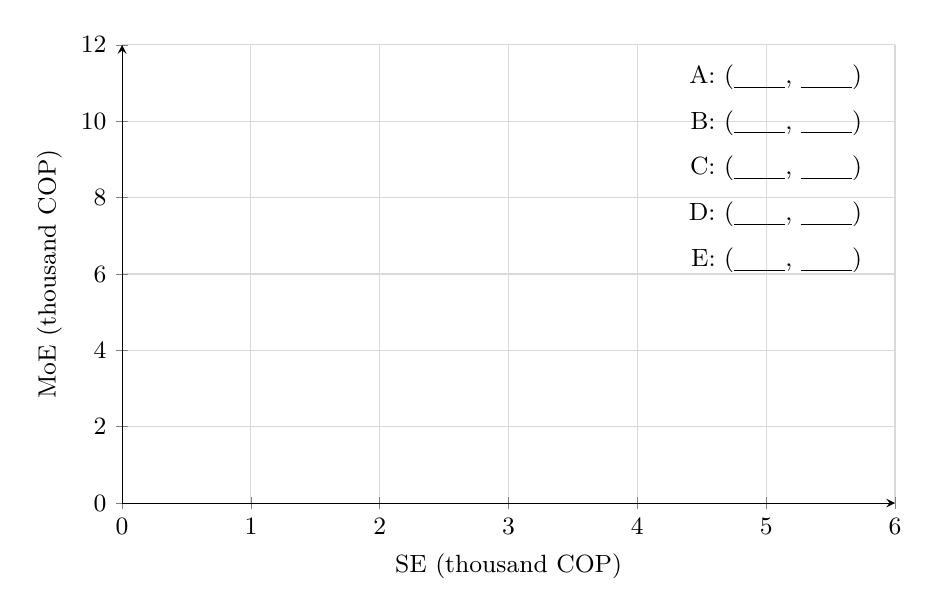
\begin{tikzpicture}\begin{axis}[relation,xlabel={SE (thousand COP)},ylabel={MoE (thousand COP)},xmin=0,xmax=6,ymin=0,ymax=12]
\LabelTemplates
\end{axis}\end{tikzpicture}\end{minipage}
\hfill\workarea\par
\clearpage
\textbf{Problem 5 --- Monthly internet costs continued}
\task{Task 2:}{Illustrate the relationships between confidence level, critical value, and margin of error.}
Hold $n=196$ and $\sigma=35$ thousand COP fixed, so $\mathrm{SE}=\sigma/\sqrt n$ stays fixed. Assume a simple random sample of independent observations from a much larger population, known population SD, and a normal population or approximately normal sample mean.
Use $\mathrm{MoE}=z^*\times\mathrm{SE}$. Cases A--E are the five supplied pairs below; the ID stays the same across all three graphs. MoE uses thousand COP; $z^*$ is unitless and $C$ is a percentage.
\begin{datagrid}{|l|X|X|X|X|X|}ID&A&B&C&D&E\\\hline $C$ (\%)&80&90&95&99&99.9\\\hline $z^*$&1.282&1.645&1.960&2.576&3.291\\\hline\end{datagrid}
Complete the three relationship graphs with five labeled points and the relationship curves. Use true numerical spacing, including near 100\%. Retain unrounded intermediate values; write calculated coordinates to three decimals. The workspace is for calculations within this task.
\par\smallskip
\begin{minipage}[t]{.49\linewidth}\vspace{0pt}\centering\textbf{Confidence level vs margin of error}\par\smallskip
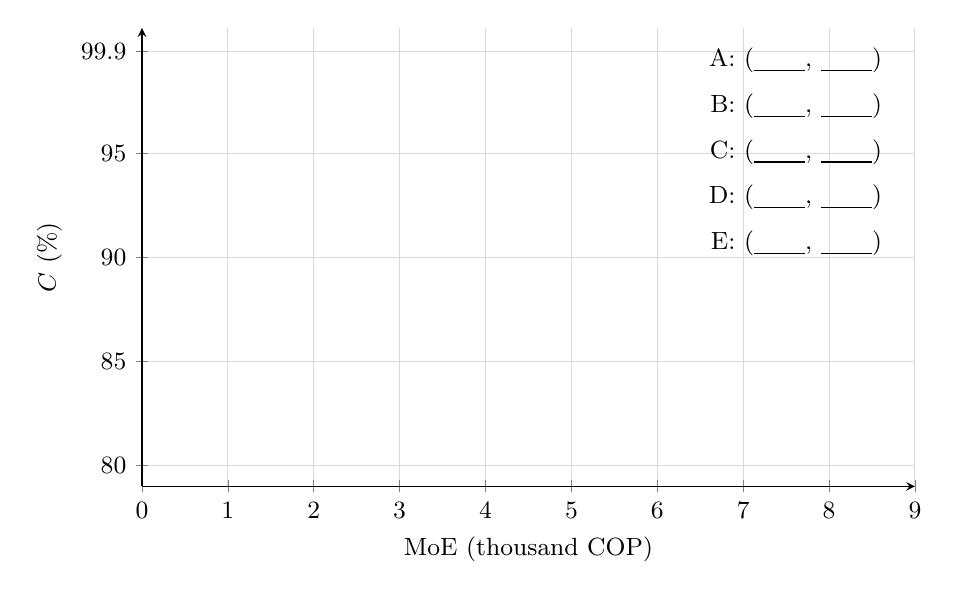
\begin{tikzpicture}\begin{axis}[relation,xlabel={MoE (thousand COP)},ylabel={$C$ (\%)},xmin=0,xmax=9,ymin=79,ymax=101,ytick={80,85,90,95,99.9}]
\LabelTemplates
\end{axis}\end{tikzpicture}\end{minipage}
\hfill
\begin{minipage}[t]{.49\linewidth}\vspace{0pt}\centering\textbf{Critical value vs margin of error}\par\smallskip
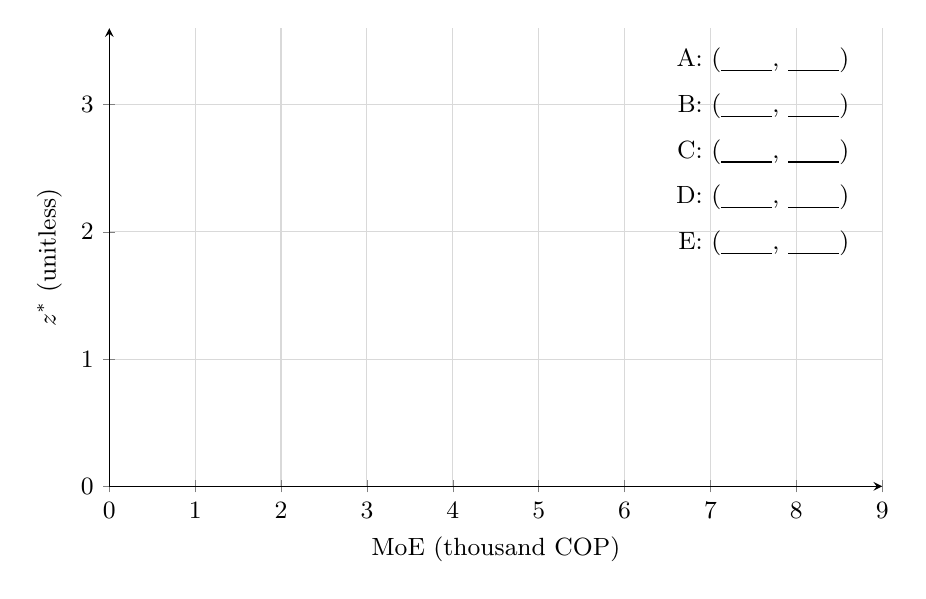
\begin{tikzpicture}\begin{axis}[relation,xlabel={MoE (thousand COP)},ylabel={$z^*$ (unitless)},xmin=0,xmax=9,ymin=0,ymax=3.6,ytick={0,1,2,3}]
\LabelTemplates
\end{axis}\end{tikzpicture}\end{minipage}
\par\medskip
\begin{minipage}[t]{.49\linewidth}\vspace{0pt}\centering\textbf{Confidence level vs critical value}\par\smallskip
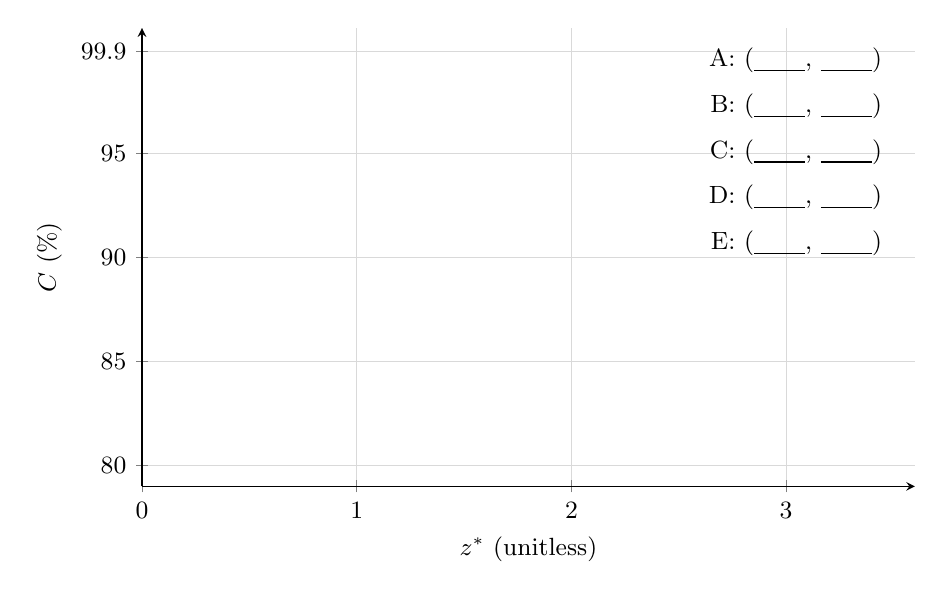
\begin{tikzpicture}\begin{axis}[relation,xlabel={$z^*$ (unitless)},ylabel={$C$ (\%)},xmin=0,xmax=3.6,ymin=79,ymax=101,xtick={0,1,2,3},ytick={80,85,90,95,99.9}]
\LabelTemplates
\end{axis}\end{tikzpicture}\end{minipage}
\hfill\workarea\par
\end{document}